\documentclass{ws-ijmpa}
\usepackage[super,compress]{cite}
\usepackage{graphicx}




\usepackage[USenglish]{babel}			 

\usepackage[final]{pdfpages}
\usepackage{multirow}
\usepackage{ragged2e}



% command for typesetting a \section like word
\newcommand\SEC[1]{\textbf{\uppercase{#1}}}


\begin{document}

\title{SixTrack project: status, runtime environment, and new developments\footnote{Research supported by the HL-LHC project}}

\title{SixTrack 5 and runtime environment\thanks{Research supported by the HL-LHC project}}

\author{
R.~De Maria \footnote{riccardo.de.maria@cern.ch},
J.~Andersson,
V.K.~Berglyd Olsen,
L.~Field,
M.~Giovannozzi,
P.~D.~Hermes,
N.~H\o imyr, \\
S.~Kostoglou,
G.~Iadarola,
E.~Mcintosh,
A.~Mereghetti,
J.~Molson,
D.~Pellegrini,\\
T.~Persson,
M.~Schwinzerl,
CERN, Geneva, Switzerland \\
E.H.~Maclean, CERN, Geneva, Switzerland and University of Malta, Msida, Malta\\
K.N.~Sjobak, CERN, Geneva, Switzerland and University of Oslo, Oslo, Norway\\
I.~Zacharov, EPFL, Lausanne, Switzerland \\
S.~Singh, IIT Madras, India \thanks{Work supported by Google Summer of Code 2018}
}
\maketitle

%\todo[inline]{remove package todonotes before submitting}

%
\begin{abstract}
SixTrack is a single-particle tracking code for high-energy circular accelerators routinely used at CERN for the Large Hadron Collider (LHC), its luminosity upgrade (HL-LHC), the Future Circular Collider (FCC), and the Super Proton Synchrotron (SPS) simulations. The code is based on a 6D symplectic tracking engine, which is optimised for long-term tracking simulations and delivers fully reproducible results on several platforms. It also includes multiple scattering engines for beam-matter interaction studies, as well as facilities to run integrated simulations with FLUKA and GEANT4. These features differentiate SixTrack from general-purpose, optics-design software like MAD-X. The code recently underwent a major restructuring to merge advanced features into a single branch, such as multiple ion species, interface with external codes, and high-performance input/output (XRootD, HDF5). This restructuring also removed a large number of build flags, instead enabling/disabling the functionality at run-time. In the process, the code was moved from Fortran 77 to Fortran 2018 standard, also allowing and achieving a better modularization. Physics models (beam-beam effects, RF-multipoles, current carrying wires, solenoid, and electron lenses) and methods (symplecticity check) have also been reviewed and refined to offer more accurate results. The SixDesk runtime environment allows the user to manage the large batches of simulations required for accurate predictions of the dynamic aperture. SixDesk supports CERN LSF and HTCondor batch systems, as well as the BOINC infrastructure in the framework of the LHC@Home volunteering computing project. SixTrackLib is a new library aimed at providing a portable and flexible tracking engine for single- and multi-particle problems using the models and formalism of SixTrack. The tracking routines are implemented in a parametrized C code that is specialised to run vectorized in CPUs and GPUs, by using SIMD intrinsics, OpenCL 1.2, and CUDA technologies. This contribution presents the status of the code and an outlook on future developments of SixTrack, SixDesk, and SixTrackLib.
\end{abstract}

\section{Introduction}
SixTrack~\cite{manual,sixweb} is a 6D single-particle symplectic tracking code able to compute the trajectories of individual relativistic charged particles in circular accelerators for studying dynamic aperture (DA) or evaluating the performance of beam-intercepting devices like collimators~\cite{roderik_samereport}. It can compute linear and non-linear optics functions, time-dependent effects, and extract indicators of chaos from tracking data. SixTrack implements scattering routines and aperture calculations to compute ``loss maps'', i.e., leakage from collimators as a function of longitudinal position along the ring, and collimation efficiency~\cite{collimat}. 

Different from a general-purpose code like MAD-X~\cite{madx, madxICAP18}, SixTrack is optimised for speed and numerical reproducibility. It can be also linked with the BOINC library~\cite{BOINC} to use the volunteering computing project LHC@Home~\cite{lhcathome}.
SixTrack studies, such as estimation of dynamic aperture of large storage rings like the Large Hadron Collider (LHC) or the Future Circular Collider (FCC), require massive computing resources, since they consist of scans over large parameter spaces for probing non-linear beam dynamics over long periods.

The SixDesk runtime environment manages SixTrack simulations from input generation, job queue management (using HTCondor or LSF in the CERN BATCH service and customised software in CERN Boinc server), to collecting and post-processing results.  

SixTrackLib is a new library built from scratch in C with the main aim of offering a portable tracking engine for other codes and offloading SixTrack simulation to GPUs.

This paper summarises the main existing features of SixTrack, SixDesk and SixTrackLib and provides details about the main development lines.

\section{Main features}

SixTrack tracks an ensemble of particles defined by a set of coordinates through several beam-line elements, using symplectic maps~\cite{ripken95, heinemann95, barber87}, or scattering elements.

\subsection{Coordinates}
The set of coordinates is larger than the minimum needed to describe the motion. Additional variables are used to store energy-related quantities used in the tracking maps that are updated only on energy changes, which does not occur very frequently in synchrotrons in absence of radiation effects, to save computational time. Thick maps for dipole and quadrupoles also reuse the energy-dependent factors of the first- and second-order polynomial of the map that are recalculated at each energy change. Furthermore, different ion species %, such as debris from interaction with matter, 
can be tracked at the same time using an extension of the usual symplectic formalism~\cite{ions}.

Variables used internally in tracking are not canonical, however, once they are converted to canonical form, the maps are symplectic.
Different from other codes, SixTrack uses
\[
\sigma=s - \beta_0 c t
\]
as the longitudinal coordinate during tracking to avoid rounding errors associated to the relativistic $\beta$ when updating time delays in drifts and
\[
\left(\zeta=\frac{\beta}{\beta_0} \sigma, \quad \delta=\frac{P-P_0}{P_0}\right)
\]
as conjugate canonical variables in 6D optics calculations which use explicitly symplectic maps.


\subsection{Beam-line elements}

\begin{table}[ht]
    \centering
    \begin{tabular}{l|l}
        \hline
         Drift expanded & Drift exact~\cite{fjellstrom13} \\
         Single thin multipole &  Thin multiple block \\
         Thick dipole-quadrupole & Thin solenoid \\
         Accelerating cavities &  RF-multipoles~\cite{rf_multipoles}\\
         4D Beam-beam & 6D beam-beam~\cite{beam_beam}\\
         Wire~\cite{wire3} & Hollow electron lens~\cite{elens,elens3}\\
         \hline
    \end{tabular}
    \caption{Physical elements implemented in SixTrack.}
    \label{tab:tracking_elements}
\end{table}

Table~\ref{tab:tracking_elements} shows the different types of beam-line elements implemented in SixTrack. Thin multipoles are used in conjunction with the \texttt{MAKETHIN} and \texttt{SIXTRACK}  commands in MAD-X to implement symplectic integrators of thick maps.
Thin multipoles include the effect of the curvature, when present, up to the second order. The tracking maps have been recently reviewed and benchmarked against MAD-X and its optics module for consistency.

\subsection{Scattering}
SixTrack embeds the K2 scattering engine~\cite{K2,CTambascoThesis}, capable of simulating the basic scattering processes undergone by an ultra-relativistic proton in the multi-TeV range when passing through matter. The simulated processes range from ionisation energy loss and multiple Coulomb scattering to point-wise interactions like Coulomb, elastic, and inelastic events, including single diffractive scattering. Compound materials of interest for the low-impedance upgrade of the LHC collimators are implemented via averaged nuclear and atomic properties~\cite{EQuarantaThesis}. Other scattering models can be imported and made available in the SixTrack executable, such as  that of Merlin~\cite{merlin} and Geant4~\cite{geant4, MolsonIPAC17}.

A new scatter block is under development to offer a general framework for simulating scattering events in SixTrack. Currently, it supports beam scattering against a target specified as an area density distribution at a thin marker inserted into the lattice.
Internally, the scattering module supports elastic scattering through Monte Carlo sampling of experimental data from Totem. Alternatively, scattering events can be generated on the fly by Pythia8~\cite{pythia8}, in which case elastic and diffractive processes are supported.

\subsection{Optics calculations}

SixTrack contains matrix code for 5D optics calculation and a 6D tracking engine using Truncated Power Series Algebra library (TPSA \cite{tpsa}) for 6D optics calculation. The 6D tracking engine uses canonical variables and it provides a cross-check of the symplecticity of the one-turn-map. Coupled Twiss parameters (using the Mais-Ripken formalism~\cite{maisripken}) can be extracted along the lattice. The optics parameters are optionally used in the beam-beam elements for self-consistent simulations. The 6D optics module has been recently improved by removing some unnecessary ultra-relativistic approximations which introduced small symplectic errors.

\subsection{Dynamic effects}

A general functionality for dynamically-changing simulation settings on a turn-by-turn basis has been implemented~\cite{dynk,dynk2}. This allows setting magnet strengths including multipoles, RF amplitude and phase, reference energy, and beam-beam element as a function of turn number. This can be useful for a number of different studies, e.g.\  magnet snap-back in the LHC~\cite{snapback_lhc}, HL-LHC crab cavity failure scenarios~\cite{crabfail1,crabfail2,crabfail3}, studies of beam losses during energy ramp~\cite{modulation}, and hollow electron-lens modulation~\cite{elens-miriam}. The settings can be internally computed as a function of turn number, or loaded from a file. These functions are specified using a flexible language that  allows combining functions to achieve the required effect. The architecture of the functionality makes it easy to add support for new elements or new functions.

\subsection{Online aperture checking}
\begin{figure*}[!tbh]
\centering
 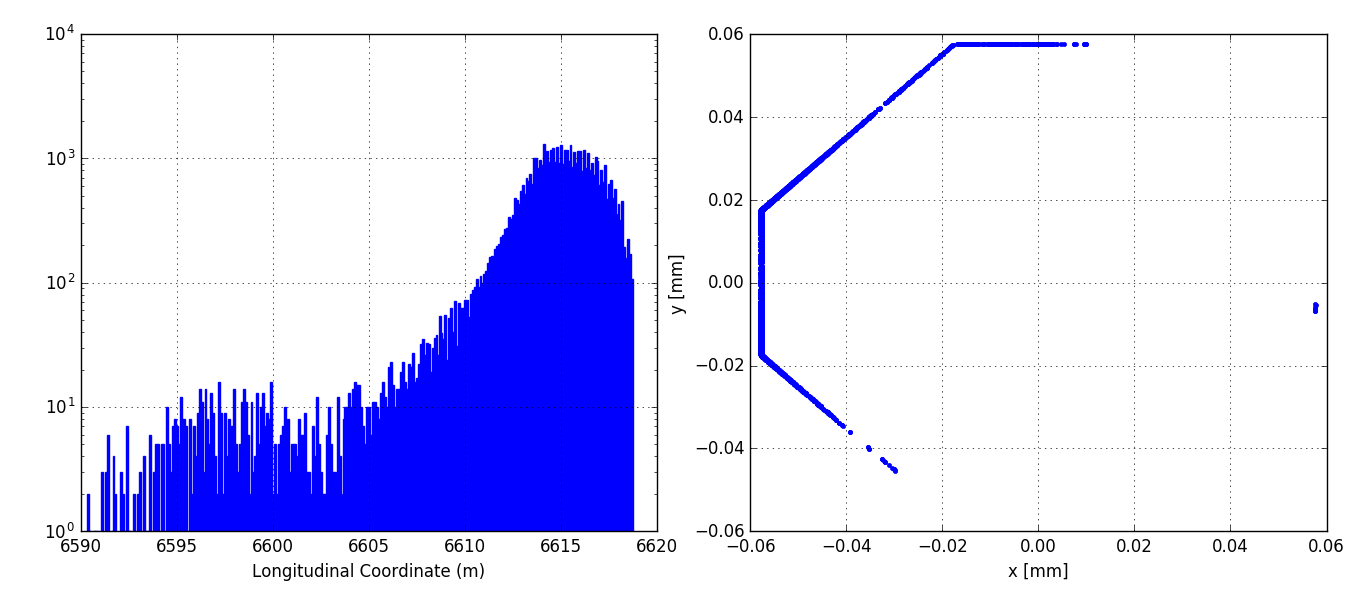
\includegraphics[width=\textwidth]{losses_IR5_mod.png}
 \caption{Longitudinal pattern (left frame) and transverse position (right frame) of losses in the inner triplet upstream of the IR5 experimental area for HL-LHC. Losses get concentrated on the upper-left quadrant (right frame) because of the local position of the closed orbit. Simulation parameters: optics v1.3, $\beta^*$=15~cm, full non-linear model of the HL-LHC (no beam-beam collisions), no collimation system.}
 \label{fig:LM_IR5}
\end{figure*}

SixTrack is capable of performing a check during tracking (online) of whether tracked particles still fall within the mechanical acceptance of the machine or not. The check is activated by the presence of aperture markers in the accelerator lattice. All aperture types of relevance for LHC, HL-LHC and FCC can be handled, namely: RECTELLIPSE (i.e.~the aperture identified by the intersection of a rectangle with an ellipse), RACETRACK (i.e.~the aperture identified by a rectangle with quadrants of ellispes at the corners) and OCTAGON. The code is capable of handling horizontal and vertical offsets of the aperture markers, as well as rotations about the longitudinal axis. The implementation comes with a smooth, linear interpolation between all supported aperture markers, such that the aperture is very well defined at any location along the ring.

A smooth linear interpolation of the aperture model of the machine is essential to the detailed identification of the actual loss point tracked particles hitting the mechanical aperture of the machine (back-tracking alghorithm). The loss location is identified comparing particle trajectories with the aperture model of the machine by means of a bi-section method; the user can set the precision of the identification of the longitudinal position. For the time being, the feature is available only for thin-lens tracking, where back-tracking is comfortably performed along a drift; extension to all other thick-lens linear elements is in plan. As an example, Fig.~\ref{fig:LM_IR5} shows the longitudinal pattern and transverse position of losses in the inner triplet upstream of the IR5 experimental area for HL-LHC~\cite{HL-TDR}; losses coming from dynamic aperture in absence of collimation system.

\subsection{Electron Lenses}
Electron lenses can be deployed to deplete over-populated beam tails in a controlled manner; as such, they are currently being investigated in the framework of the HL-LHC project~\cite{HL-TDR}. The module is in continuous development~\cite{elens-miriam}. Recent changes include: porting to ion tracking, relevant for benchmarking recent measurements at RHIC~\cite{RHIC-Mirarchi}; possibility to deploy measured radial profiles of electron beams; compatibility to the BOINC platform for volunteering computing, relevant for evaluating long-term effects on dynamic aperture. On-going development is focussed on implementing 2D maps of measured electron profiles by means of Chebyshev polynomials~\cite{GStancari-Chebyshev}.

\subsection{Post processing}
\begin{figure}[tbh]
\centering
 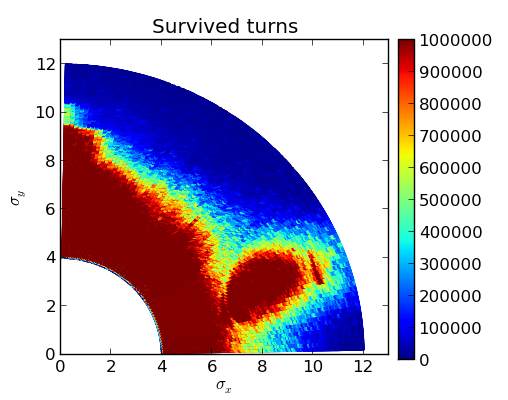
\includegraphics[width=\columnwidth]{surv_plot1.png}
 \caption{Survival plot of a fine phase-space scan for the LHC. The simulations was divided in task of $60$ particles pairs covering the phase space in $2\sigma$ and $1.5^\circ$ steps.}
 \label{fig:study}
\end{figure}

Long-term tracking with SixTrack is used extensively at CERN for studying the DA, with a typical study consisting of up to $\sim 2\times 10^{6}$ individual tracking simulations over $10^5-10^6\,\mathrm{turns}$ (see Figure \ref{fig:study} for an example).

Tracking data are post processed during the study and summary files, containing the main results of the simulation for each initial condition, are returned back to the user. In particular, tracking summary files for each initial condition identify particle loss/survival, final surviving turn numbers and the inferred particle amplitudes.

Particle's invariants are calculated for each initial condition and based on the average invariant over a user-defined range of turns.
An initial estimate of the invariant is obtained by assuming no coupling between the planes of motion, via the usual relation for the Courant-Snyder ellipse, e.g.\ for the horizontal plane.
Alternatively, an estimate of the decoupled single-particle emittance for the three oscillation modes can be calculated from the eigenvectors of the motion ($\bar{v}$), which may be constructed from the one-turn map, see for example~\cite{maisripken}. Various parameters relevant to the nonlinear motion, such as smear and detuning, are also evaluated.

In addition to quantities relevant to particle survival, estimates of the long-term stability are obtained through a Lyapunov-like analysis performed by examining the phase-space separation of initially close by particle pairs. In particular, the angular separation in phase for the three oscillation modes
\begin{align}
&\frac{1}{\pi}\sqrt{\frac{ \Delta\phi_{1}^2 + \Delta\phi_{2}^2 + \Delta\phi_{3}^2 }{N}}&\nonumber
\end{align}
where $N=(1,2,3)$ for $(2D,4D,6D)$ motion, respectively, is considered. Linear fits to the logarithm of the separation as function of the logarithm of the turn number identify the maximum separation rate between each particle pair. This quantity is returned, along with the maximum separation in phase, to provide approximate indicators of the onset of chaotic motion in place of the far more computationally intensive Lyapunov exponents~\cite{chaosproxy,distanceslope}.

Summary files for the outcome of each initial condition are collectively post-processed by the user using external tools, in order to identify minimum boundaries in the $(\sigma_{x},\sigma_{y})$ space for particle survival over the tracked number of turns, as well as to study the evolution of DA as a function of the turn number.

\subsection{Frequency analysis}

A collection of routines for frequency analysis has been linked in SixTrack, namely PLATO~\cite{plato} and a C++ implementation of the Numerical Analysis of Fundamental Frequency (NAFF) algorithm has been developed~\cite{naff}. These algorithms allow for a more refined, compared to plain FFT, tune determination with a much faster convergence, i.e. requiring a shorter number of turns. By comparing the tune determination at different time intervals,  diffusive frequency maps can be been computed~\cite{laskar}. With the resolution of the frequency map, resonance lines become visible, even in the case of a tune modulation from a quadrupolar ripple (the triplets in IR1 and 5) with frequency of $550$~Hz and relative amplitude of $10^{-7}$, as shown in Figure~\ref{fig:fma}.

\begin{figure*}[!tbh]
\centering
 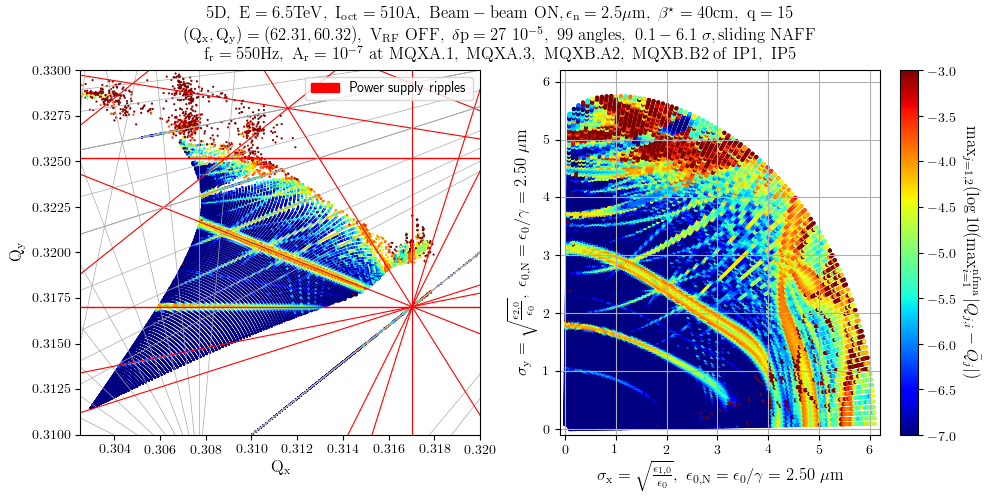
\includegraphics[width=\textwidth]{FMA.png}
 \caption{Frequency map using the NAFF method for LHC in the presence of a tune modulation.}
 \label{fig:fma}
\end{figure*}

\subsection{Input and output}

Initial conditions can be given in amplitude steps or taken from an external file. A dump module offers multiple ways to extract tracking data both in terms of type observable (physical coordinates, canonical coordinates, normalised coordinates, averages and first order distribution momenta) in a selection of turns and observation points. Data are written in ASCII and, in a few cases, a binary option is also available. Support for output of simulation data to a HDF5~\cite{hdf5} files and ROOT~\cite{root} is also currently being developed.

Furthermore, it is planned to develop a new way to generate the distribution that is used as initial conditions for tracking. This will provide the functionality to create matched or mismatched distributions in both physical and normalised coordinates.

\subsection{Interfaces to external programs}

Collimation studies can also be performed running SixTrack coupled~\cite{flukaCouplingVV} to Fluka~\cite{FLUKA1,FLUKA2}. In this configuration, the two codes exchange particles at run time, with the aim of combining the refined tracking through the accelerator lattice, performed by SixTrack, with the detailed scattering models, implemented in Fluka, when the beam reaches intercepting devices. The use in the Fluka-SixTrack coupling of the same Fluka geometries used for subsequent energy-deposition calculations run with Fluka allows an excellent level of consistency of results.

\begin{figure*}[!tbh]
\centering
 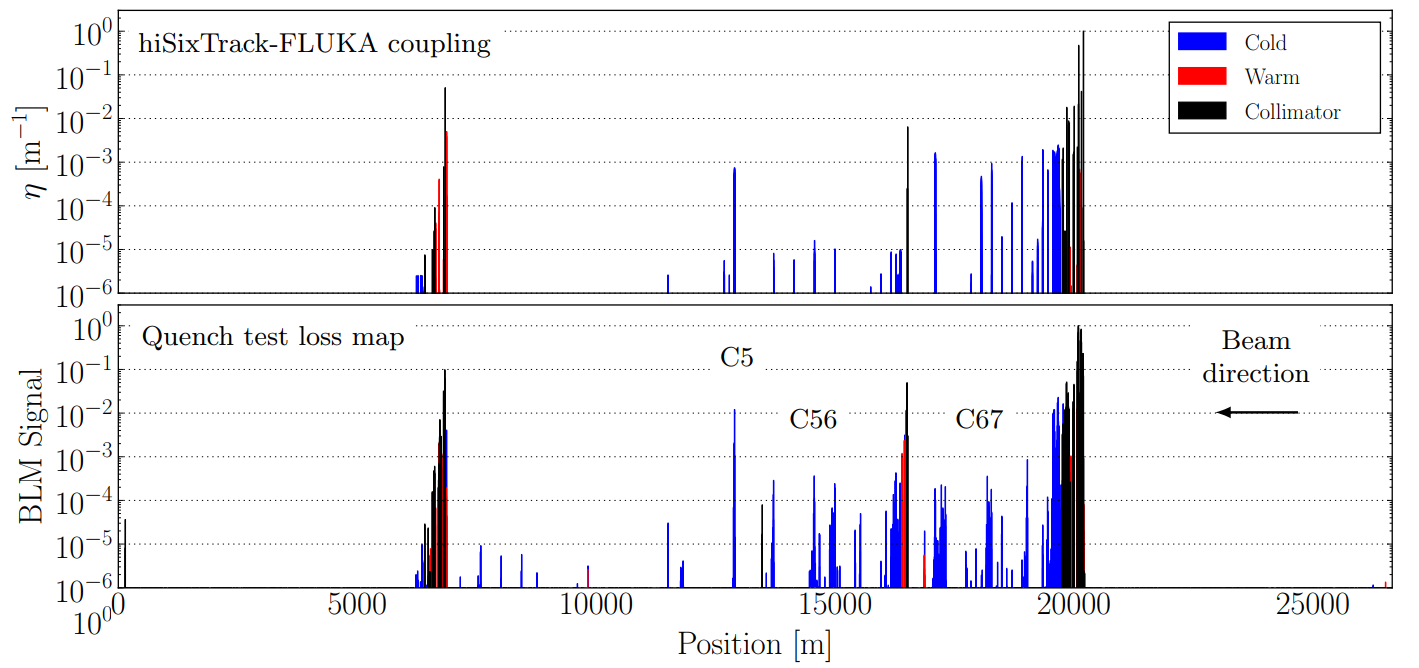
\includegraphics[width=\textwidth]{QT_LHC_mod.png}
 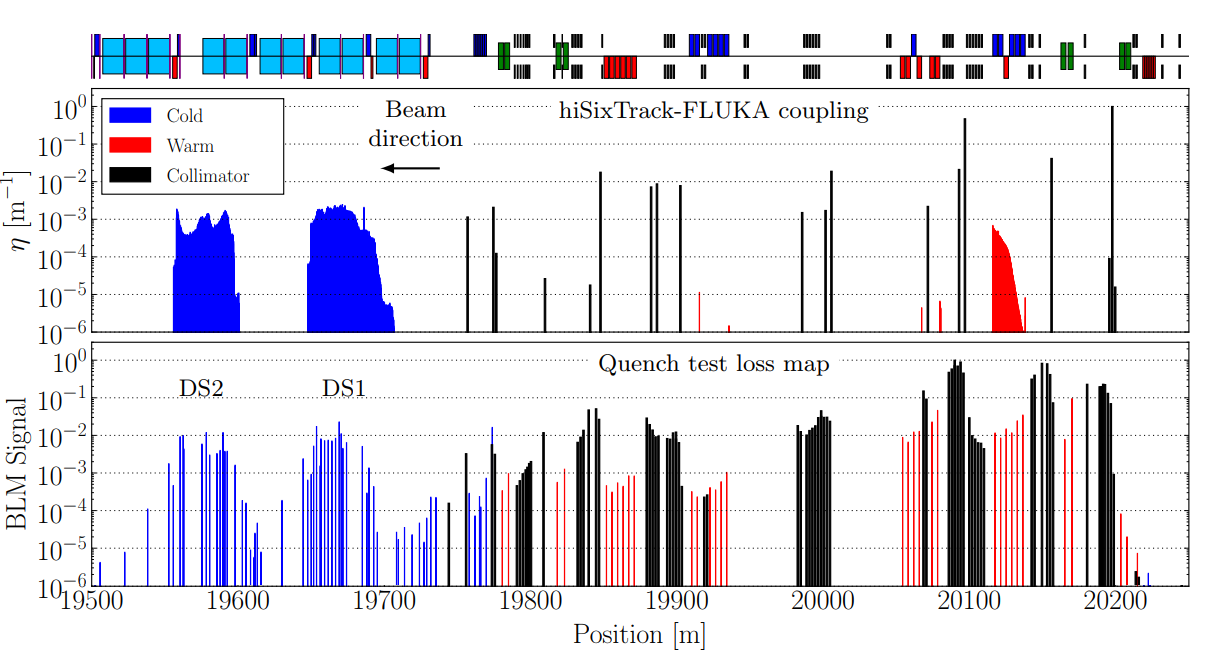
\includegraphics[width=\textwidth]{QT_IR7_mod.png}
 \caption{Comparison between losses predicted by the SixTrack-Fluka coupling and measured by beam loss monitors during the ion collimation quench test in 2015~\cite{PDHermes-PhD}. Losses around the ring (upper frame) and zoom in the region of the collimation insertion dedicated to betatron cleaning at the LHC.}
 \label{fig:QT_LMs}
\end{figure*}
%\begin{figure}[tbh]
%\centering
% 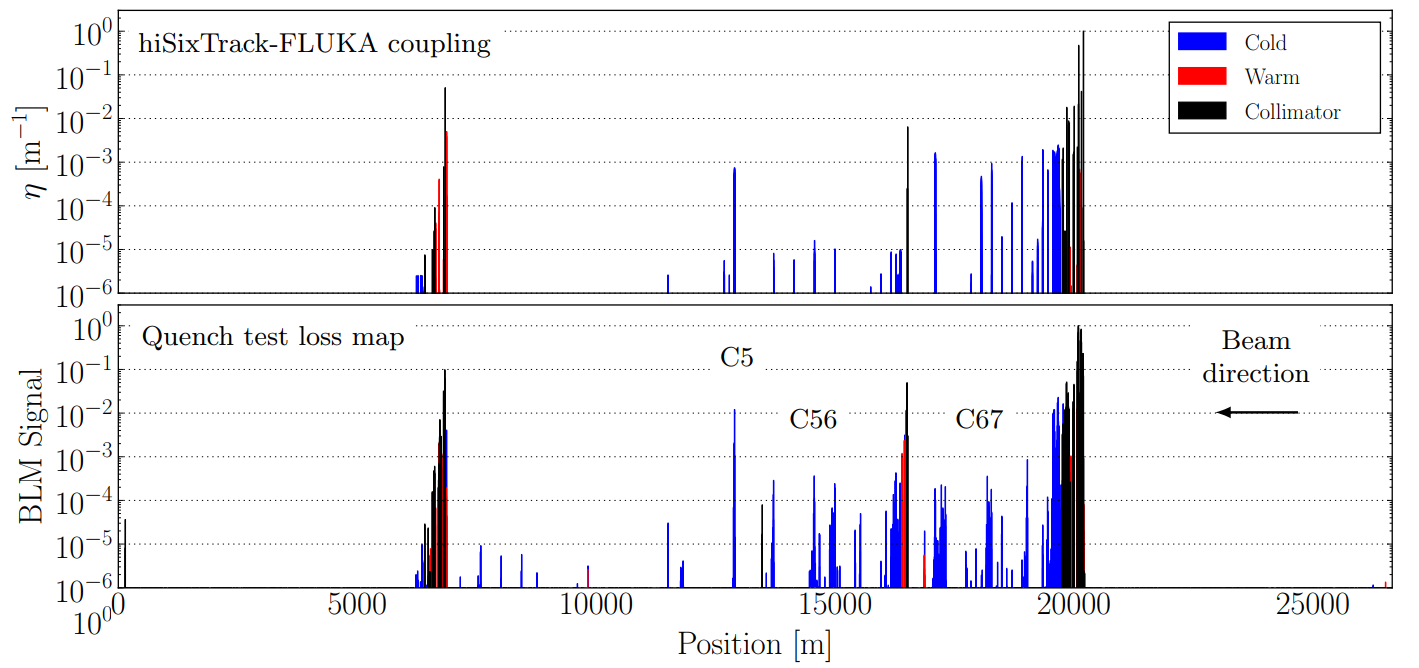
\includegraphics[width=\columnwidth]{QT_LHC_mod.png}
% 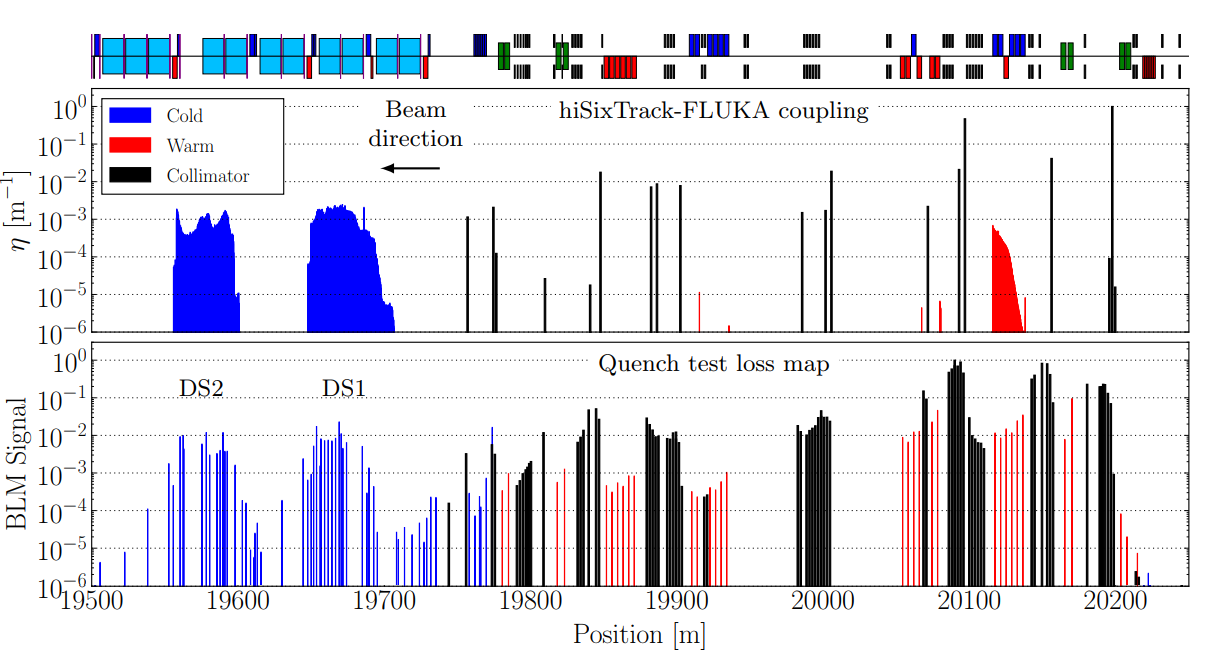
\includegraphics[width=\columnwidth]{QT_IR7_mod.png}
% \caption{QT.}
% \label{fig:QT_LMs}
%\end{figure}
As an example, Fig.~\ref{fig:QT_LMs} compares the losses around the ring as predicted by the Fluka-SixTrack coupling and as measured by beam loss monitors during the ion collimation quench test in 2015~\cite{PDHermes-PhD}. The test aims at artificially generating high losses in the cold region of the machine in a controlled way to probe margins to quench (i.e.~the change of state from superconducting to normal conducting). Simulations are an essential ingredient to estimate the energy deposition in the superconducting coils at the origin of the quench. Simulations accurately predict the main loss points and the relative loss intensities; for a more quantitative benchmark, detailed Fluka simulations should be run in order to estimate the BLM signal with the simulated losses and the energy deposition in the cold mangets.

Additionally, a more generalised interface ``BDEX'' for interfacing external codes is also included, enabling for example tracking of multiple bunches or coupling to cavity simulation codes.
Here, the exact protocol can be implemented as a plug-in to SixTrack~\cite{recentDevels2}.

%A more generalised interface ``BDEX'' for interfacing external codes has also been developed~\cite{recentDevels2}. This is capable of exchanging or exporting the tracked particle distribution at any marker. The protocol for the particle exchange is flexible, allowing addition of new protocols as needed. Currently, only an ASCII-based protocol, intended to be used with UNIX pipes, is supported. The functionality has previously been used (together with DYNK's functionality to communicate with external programs) to track whole HL-LHC trains, swapping out the bunch at a point along the ring. Additionally, the code was also coupled to an external collective-effects model for computing beam loading in the crab cavities, where the effect of each bunch passing through the cavity as well as the response of the RF system was applied to the next bunch {\bf I would add a refernce here.}.

\subsection{Building and testing}

A CMake-based build and test system has recently been added~\cite{recentDevels2}. This greatly simplified the maintenance of the dependencies between the various build options, as well as the setup for building on the large range of supported platforms.

The testing framework CTest is also provided as part of CMake. For SixTrack, this is used to verify that the executables are still providing the expected output after the code has been modified, and to track the changes to the output. Furthermore, it is used for checking that the results from versions compiled for different platforms are in agreement, which is vital for BOINC. The main benefit of using CTest is that test running is fully automatic and gives a simple pass/fail output, which is also integrated with GitHub for pull requests.

\subsection{Performance}

Thanks to the recent re-factoring, the internal particles arrays are fully dynamic, therefore the number of particles that can be tracked in parallel is limited by the system memory and not by a build-time flag. A machine model like the LHC, using about $18$k elements and $4.6$k high-order multipole blocks, needs about $220$~\textmu s per particle per turn on a single CPU core at 3.4~GHz. Typical studies requires of the order of $10^9 - 10^{12}$ particle turns and even more for parameter scans. For this reason, SixTrack is often used in conjunction with high-performance computing facilities described in the following section.

\section{Runtime environments}

The SixDesk environment~\cite{sixdesk} is the simulation framework used to manage and control the large amount of information necessary for, and produced by, SixTrack studies of dynamic aperture. It supports CERN batch systems~\cite{cernbatch} as well as the BOINC platform for volunteering computing available at the LHC@Home project~\cite{lhcathome}. The SixDeskDB post-processing tool collects data from SixDesk, performs post-processing analysis, and prepares reports and plots. It also offers a Python API for interactive analysis. Similarly to the SixTrack code, the SixDesk environment and SixDeskDB are continuously updated, extending the coverage of the studies and keeping the environment up to date with the latest developments in the CERN IT infrastructure.



\begin{figure*}[tbh]
\centering
 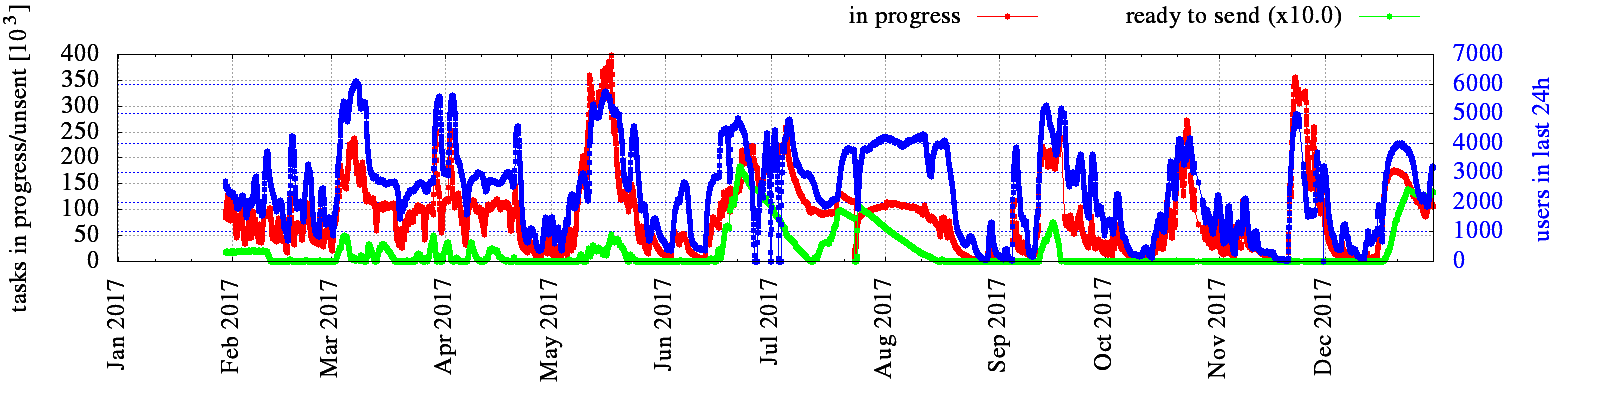
\includegraphics[width=\textwidth]{sixtrackOverview_2017.png}
 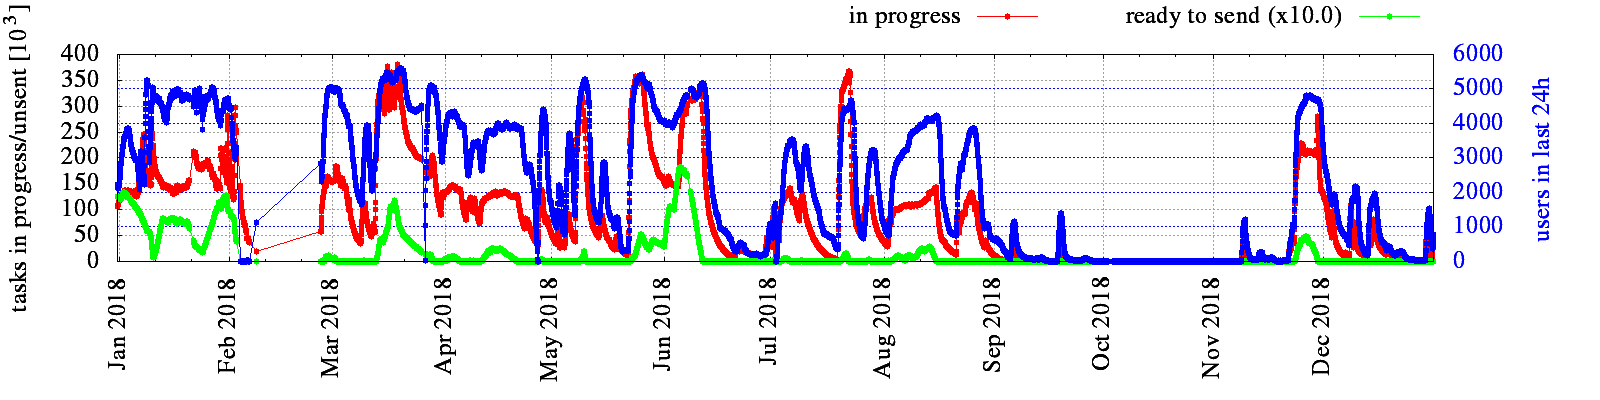
\includegraphics[width=\textwidth]{sixtrackOverview_2018.png}
  \caption{Summary of tasks and users during the last two years (upper frame: 2017; lower frame: 2018 to date) of the SixTrack application in the LHC@Home project. The number of users tends to increase, with the number of tasks absorbing most of the time all pending tasks.}
 \label{fig:boinc}
\end{figure*}

\subsection{LHC@Home and the CERN Batch System}

Volunteer computing has been used successfully at CERN since 2004 with the LHC@Home project; it has provided additional computing power for CPU-intensive applications with small data sets, as well as an outreach channel for CERN activities. LHC@Home started off with SixTrack, which had been successively ported from mainframe to supercomputer to emulator farms and PCs. In order to run on the largest number of volunteer computers, SixTrack is compiled for the most common operating systems, architectures, and CPU instruction sets.

In terms of computing power provided by the volunteers to LHC@home, the system is capable of handling $1\times 10^5$ tasks on average, with peaks of $3.5 \times 10^5$ tasks simultaneously running on $2.4 \times 10^4$ hosts observed during SixTrack intense simulation campaigns (see Figure~\ref{fig:boinc}). Every SixTrack task is run twice to eliminate random host errors and minimise the impact of a failing host. The LHC@Home capacity available for SixTrack can be compared to the average of $2.5 \times 10^5$ running tasks on $1.4 \times 10^5$ processor cores in the CERN computer centre, which is fully loaded with tasks from analysis and reconstruction of collisions recorded by LHC experiments, and has limited spare capacity for beam dynamics simulations.

The CERN batch system is presently managed by means of the HTCondor~\cite{HTCondor} package. Contrary to BOINC, most suitable for a steady stream of work units, the CERN batch system provides users with a responsive computing resource. Also, contrary to LHC@Home, no redundancy is implemented during task submission since the code run in a controlled environment, although very rarely hardware errors do appear in the results.

\subsection{Developments}

One of the main development lines of SixDesk is porting the collimation studies to the BOINC platform for volunteer computing. This entailed a thorough revision of the collimation part, currently on-going, to make results numerically stable and reproducible across platforms. The possibility to interrupt and restart the computation (check-point/restart capability), which is essential to run on BOINC,  is being added as well.

Other lines of development include: the addition of new parameters for dedicated scans of dynamic aperture; the possibility of running chains of jobs in BOINC, for simulating extended periods of beam time in the ring; a pre-filtering stage of submission to the CERN batch system prior to submission to BOINC, to avoid short tasks, with consequent inefficient use of volunteer resources, like bandwidth and time.

\section{SixTrackLib}
In the context of single-particle simulations, tracking requires no interaction between the calculations carried out for particle $p_i$ and $p_{j\neq i}$ from a set of $N$ 
particles. The memory requirements for representing each $p_i$ typically ranges from $10^1$ to $10^3$ Bytes. The machine description can, over a single turn, be considered 
constant, although different elements and sections of the ring require a different amount of local resources. Still, SixTrack presents itself as an ideal candidate for a 
parallel implementation; in fact, strongly CPU bound with inherent parallelism and resource requirements not inherently scaling with the number of parallel processes. 

Introducing parallelism into a mature code-base like SixTrack, even from such a favourable starting point, is challenging. It entails a high level of complexity due to 
competing paradigms and concepts of parallel computing. In particular, a fast-changing technological landscape in combination with a diverse, multi-vendor and long-tailed 
selection of hardware available via initiatives like LHC@Home~\cite{lhcathome}, as well as the realities of limited development resources are the main decision-making factors. 
These and other constraints motivated the design and ongoing development of SixTrackLib~\cite{sixtracklib}, a clean-room implementation of the core functionality of SixTrack as
a stand-alone library, allowing users to off-load the task of particle tracking onto supported HPC resources. The library provides 
\begin{enumerate}[label=(\alph*)]
 \item a representation for a set of particles 
 \item a set of beam-elements such as drifts, magnetic multipoles (e.g. dipoles, quadrupoles, sextupoles, etc.), RF cavities, $4D$ and $6D$ beam-beam elements, etc\ldots 
 \item a set of maps describing the tracking of particles over the beam-elements
 \item a beam monitor lattice element, allowing to represent the functionality of beam instrumentation devices such as beam-position monitors, beam-profile monitors, etc.
 \item a range of contexts representing different parallelism and high-performance paradigms (e.g. auto-vectorized CPU code, OpenCL~\cite{opencl}, CUDA~\cite{cuda}) and the 
       associated computing nodes within these paradigms
 \item a dedicated generic buffer for managing collections of particles, beam elements and for transfer data to and from and the computing nodes 
 \item a set of high-level APIs in C, C++ and (under development) Python.
\end{enumerate}

The design of the library aims to completly separate the parts containing the physics (i.e. the particles, the beam elements, and the tracking maps) in a header-only module usable from C-like languages (e.g. C, C++, Cuda, OpenCL, etc.) 
from the platform specific implementation pertinent to different computing environments and paradigms. Expressing the components in the abstracted header-only physics module allows the reuse of the modelled physics across all 
supported computing paradigms and to easily tap into the functionality of the tracking library from concrete and already existing applications and frameworks. Another benefit of this approach is the ability extend the physics (for example 
by adding additional or alternative implementations for beam-elements) without the need to address different computing backends (or, vice versa, being able to add support for additional HPC environments without having to revisit the 
existing collection of physics related code-paths). The use of automatically generated code to aid users in such scenarios and to improve the maintainability of the code by reducing the libraries footprint in terms of lines-of-code is currently under development.  

SixTrackLib is developed in concert with pysixtrack~\cite{pysixtrack}, a reference implementation of the SixTrackLib physics using pure Python. It focuses on a straight forward and easy to understand version of the modelled physics, numerical reproducibility and numerical precision (by virtue of allowing the use of extended precision numerical types present in python) rather than performance or scalability. By comparing results between pysixtrack, SixTrackLib and SixTrack, the feasibility of the chosen design, the numerical accuracy and the performance can be evaluated and quality assured as part of the test-driven development efforts.
 
Consider for example a simulation on a lattice representing the LHC over a sequence of $100$ turns while comparing the results generated via SixTrackLib against pysixtrack (Fig.~\ref{fig:cmp_sixtracklib_pysixtrack}) and SixTrack (Fig.~\ref{fig:cmp_sixtracklib_sixtrack}). 
\begin{figure}[htb]
 \centering
 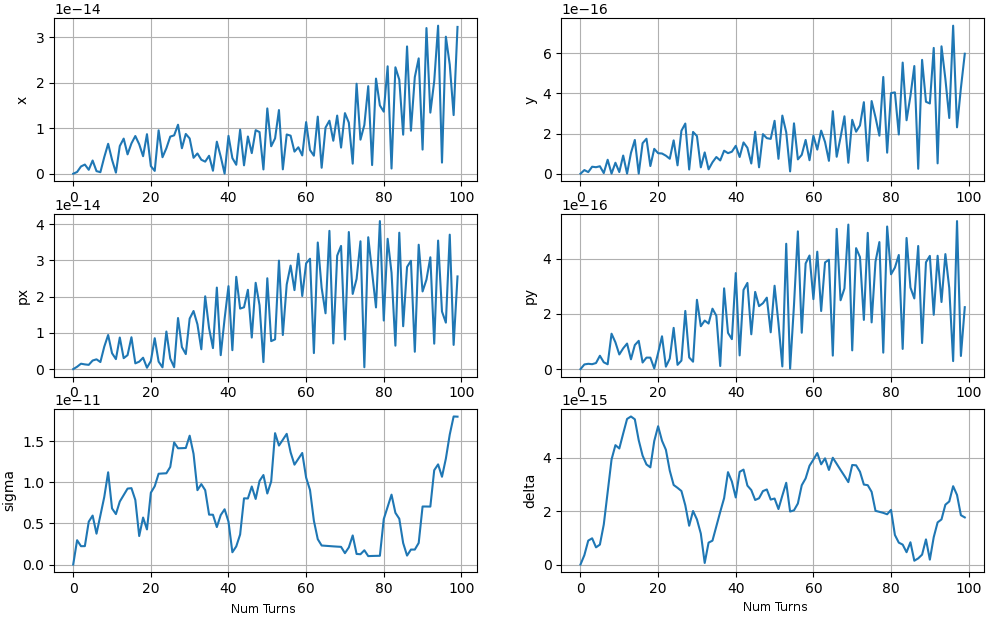
\includegraphics[width=\columnwidth]{cmp_sixtracklib_pysixtrack.png}
 \caption{Absolute numerical difference of SixTrackLib and pysixtrack simulations of the LHC lattice over 100 turns.}
 \label{fig:cmp_sixtracklib_pysixtrack}
\end{figure}
\begin{figure}[htb]
 \centering
 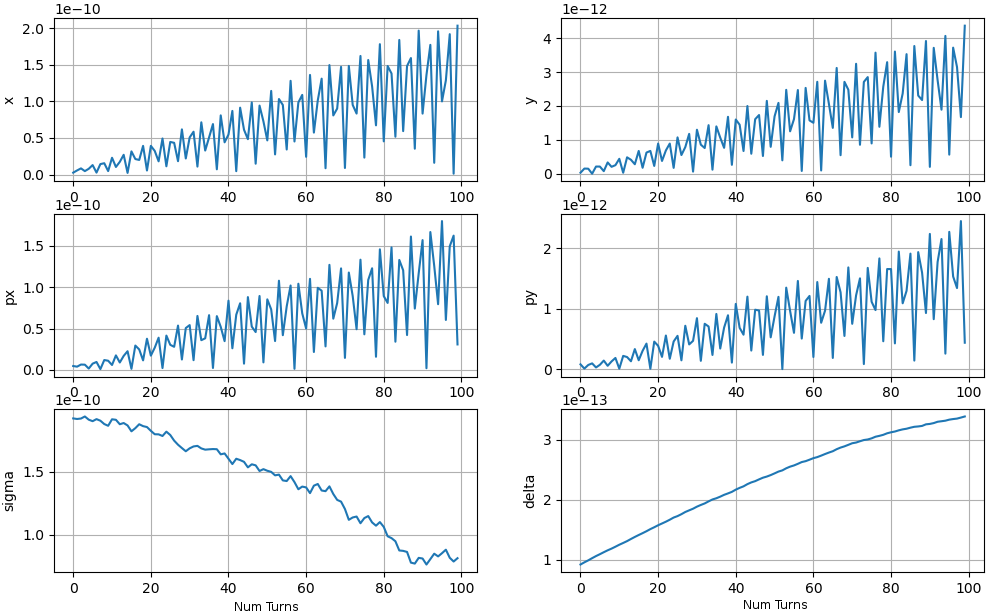
\includegraphics[width=\columnwidth]{cmp_sixtracklib_sixtrack.png}
 \caption{Absolute numerical difference of SixTrackLib and SixTrack simulations of the LHC lattice over 100 turns.}
 \label{fig:cmp_sixtracklib_sixtrack}
\end{figure}
The presented magnitude of the absolute numerical difference in each of the six degrees of freedom is within admissible limits to prove the feasibility of the chosen desgin of both SixTrackLib and pysixtrack and lays the ground-work for further investigations and optimizations into this aspect. 

Concerning an evaluation of the performance improvements achievable by using the parallel hardware capabilities of CPUs and GPUs via SixTrackLib and given the inherent parallelism of the problem outlined above, the main limiting factors for achieving high scalability and numerical throughputs are expected to be a)~the finite availability of resources such as registers and high-bandwidth/low-latency memory on computing nodes and 
b)~the ability to compensate for any occurring latencies by having enough parallel tasks scheduled to prevent computing units from stalling or idling. 

In order to study the impact of these effects, it is illustrative to simulate the same lattice using different transfer maps resulting in the same physics but requiring differnt amounts of hardware resources, (e.g. registers). The by far most demanding transfer maps present in SixTrackLib as of this writing are the $4D$ and $6D$ beam-beam interaction implementations. By comparing the performance of simulating a lattice without beam-beam interactions once with a streamlined set of maps online during the simualtion and once with passive (i.e. unused) support for beam-beam interactions available, the effect can be illustrated and its impact in real-world scenarios estimated.

Consider to this end the simulation of $1 \leq N \leq 10^7$ particles on a lattice representing the LHC without beam-beam interactions using SixTrackLib, as presented in (Fig.~\ref{fig:sixtracklib_results}). 
Evaluating the impact of the beam-beam maps using the OpenCL backend is especially interesting as it allows to directly compare the performance implications on both CPU and GPU configurations across vendors. 
The presented results encompass both CPUs (Intel Xeon E5-2630 20x2.2 GHz hyper-threads, AMD Ryzen 1950X, 16x3.40 GHz hyper-threads) and a range of both high-end GPUs (NVIDIA Tesla V100 PCIe 16GB GPU) as well as 
consumer-grade graphical processors (NVIDIA GTX 1050Ti 4GB, AMD RX560 4GB). The results demonstrate parallel speed-ups approaching (for large $N$) factors of $10^1$ to and exceeding $10^2$. 
\begin{figure}[htb]
 \centering
 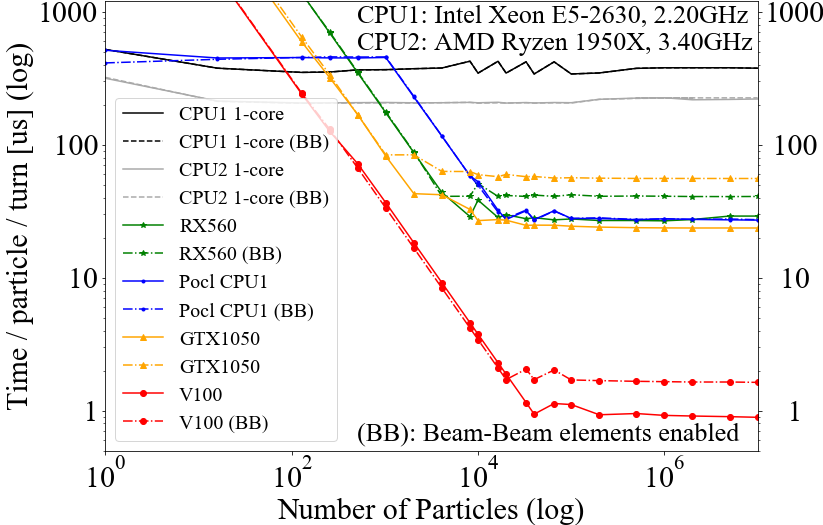
\includegraphics[width=\columnwidth]{devices_times_per_particle_and_turn.png}
 % devices_times_per_particle_and_turn.png: 841x595 px, 72dpi, 29.68x21.00 cm, bb=0 0 841 595
 \caption{Benchmarking results of a LHC study using SixTrackLib on different target hardware. Increasing the complexity of the parallel code by enabling beam-beam elements (BB), but not using them, leads to decreased performance on GPUs, but not on CPU-based systems.}
 \label{fig:sixtracklib_results}
\end{figure}

The impact of passivley enabling the beam-beam interactions (labeled using (BB) in Fig.~\ref{fig:sixtracklib_results}) in the parallel tracking code leads, unsurprisingly, to virtually no change on CPU-based systems; these systems are not as sensitive to register pressure and resource starvation as graphical processor based environments. 
For the GPU based configurations, the increased complexity and pressure on resources impairs the performance on all studied systems, although the degree of the impact and the economics of keeping complex maps on-line even if the features are not actively used
are differing considerably even within the context of this limited set of considered hardware configurations. The results motivate studying ways to split the monolithic parallel code into smaller specialised blocks and to provide APIs and facilities to execute these blocks in sequence, thereby trading in synchronisation and dispatching overheads for a potentially better utilisation of hardware resources.

\section{Conclusions}

The SixTrack tracking code is the main code used to simulate long-term stability, collimation cleaning, and machine failure scenarios in the LHC, SPS and FCC due its unique features of speed and integration with HPC resources. It comes with a fully developed running environment to perform easily the massive numerical simulations that include scans on beam and ring parameters and the option of using different computing resources, from standard batch services to volunteer computing. 

In spite of its maturity, SixTrack is still in an intense development phase. On the short time scale, it is planned to merge into a single code the features that were developed in the framework of the studies of the LHC collimation system. On a longer time scale, the main lines of development include  tighter integration of existing features, interoperability with other codes, and deployment on new architectures such as GPU.

\section{Acknowledgements}

We wish to thank all volunteers that supported and continue to support the SixTrack project and the related studies by donating  to the LHC@Home Project their CPU power and technical advice. We also wish to thank F.~Schmidt for his continuous interest in SixTrack development.

\begin{thebibliography}{99}
%%%% Examples from http://www.jacow.org/Authors/FormattingCitations

%% A. Alpha and B. T. Beta, ``...'', report number, year.
%% A. Alpha {\it et al.}, ``...'', {\it Journal} {\bf issue} ... (year).
%% A. Alpha, B. T. Beta, C. Gamma, and D. Delta, ``...'', in {\it Proc~}, place, state, year, paper MO... .

\bibitem{manual}
F. Schmidt {\it et al.},
``SixTrack Version 4.2.16 Single Particle Tracking Code Treating Transverse Motion with Synchrotron Oscillations in a Symplectic Manner'',
CERN/SL/94-56, 2012.

\bibitem{sixweb}
SixTrack Project website,
\url{http://cern.ch/sixtrack}.

\bibitem{roderik_samereport}
R. Bruce {\it et al.},
``Status of Sixtrack with collimation'',
in \emph{Proc.~Tracking for Collimation Workshop}, CERN, Geneva, Switzerland, 2018.

%\bibitem{racetrack}
%A.F. Wrulich,
%``{RACETRACK}: a computer code for the nonlinear particle motion in
%accelerators,''
%DESY 84-026, 1984.

\bibitem{collimat}
G. Demolaize {\it et al.}, ``A New Version of SixTrack with Collimation and Aperture interfaces'', in {\it Proc.~PAC'05}, Knoxville, TN, USA, May 2005, paper FPAT081.

\bibitem{madx}
MAD-X Project website, \url{http://cern.ch/mad}

%\bibitem{madxICAP18} L.~Deniau, A.~Latina, T.~Persson, P.~Skowronski, H.~Burkhardt, J.M.~Jowett, F.~Schmidt, M.~Giovannozzi, ``Upgrade of MAD-X for HL-LHC project and FCC studies'', these proceedings. 

\bibitem{madxICAP18}
L.~Deniau {\it et al.},
``Upgrade of MAD-X for HL-LHC project and FCC studies'',
these proceedings.

\bibitem{BOINC} D.~P.~Anderson, ``'BOINC: a System for Public-Resource Computing and Storage',
in \emph{Proc.~of the 5$\textrm{th}$ IEEE/ACM International Workshop on Grid Computing}, Pittsburgh, USA, 2004.

\bibitem{lhcathome}
% M.\ Giovannozzi {\it et al.}, 	
% ``LHC@Home: A volunteer computing system for massive numerical simulations of beam dynamics and high energy physics events''
% in {\it IPAC'12 Proceedings}, New Orleans, LA, USA, May 2012, paper MOPPD061.
J.~Barranco \emph{et al.},
``LHC@Home: a BOINC-based volunteer computing infrastructure for physics studies at CERN'',
{\it Open Engineering} {\bf 7} 378 (2017).

\bibitem{ripken95}
G.~Ripken and F.~Schmidt,
``A symplectic six-dimensional thin-lens formalism for tracking'',
DESY 95-63, CERN/SL/95-12(AP), 1995.

\bibitem{heinemann95}
K.~Heinemann, G.~Ripken, and F.~Schmidt,
``Construction of nonlinear symplectic six-dimensional thin-lens maps by exponentiation'',
DESY 95-189, 1995.

\bibitem{barber87}
D.P. Barber {\it et al.},
``A non-linear canonical formalism for the coupled synchro-betatron motion of protons with arbitrary energy'',
DESY 87-36, 1987.

\bibitem{ions} P. Hermes {\it et al.},
``Symplectic Tracking of Multi-Isotopic Heavy-Ion Beams in SixTrack'', in \textit{Proc.~IPAC'16}, Busan, Korea, May 2016, paper TUPMW015.

%%% beam line
\bibitem{fjellstrom13}
M. Fjellstrom, ``Particle Tracking in Circular Accelerators Using the Exact Hamiltonian in SixTrack'', CERN-THESIS-2013-248, 2013.

\bibitem{rf_multipoles}
A.~Latina and R.~De Maria, ``RF multipole implementation'', CERN-ATS-Note-2012-088 TECH, 2012.

\bibitem{beam_beam}
L.H.A. Leunissen {\it et al.}, ``6D beam-beam kick including coupled motion'', {\it Phys.\ Rev.\ ST Accel.\ Beams} {\bf 3} 124002 (2000).

\bibitem{wire3}
A. Patapenka,
``First order transport map of wire element'',
in \textit{3rd General SixTrack Meeting}, 7 December 2016, \url{https://indico.cern.ch/event/590257/}.

\bibitem{elens}
V. Previtali {\it et al.},
``Numerical Simulations of a Hollow Electron Lens as a Scraping Device for the LHC'',
in \textit{Proc.~IPAC'13}, Shanghai, China, May 2013, paper MOPWO044.

%\bibitem{elens2}
%M. Fitterer, {\it et al.}, ``Electron lens news'', 3rd General SixTrack Meeting, 7th %December 2016, \url{https://indico.cern.ch/event/590257/}.

\bibitem{elens3}
M. Fitterer {\it et al.},
``Implementation of Hollow Electron Lenses in SixTrack and first simulation results for the LHC'',
in \textit{Proc.~IPAC'17}, Copenhagen, Denmark, May 2017, paper THPAB041.

%\bibitem{wire}
%A. Patapenka, ``Wire implementation in SIXTRACK'', Beam-Beam and Luminosity Studies %meeting, 3 August 2015, \url{https://indico.cern.ch/event/436670/}.

%\bibitem{wire2}
%A. Patapenka, ``Wire model in Sixtrack - simulation results,''
%in \textit{Simulations and Measurements of Long Range Beam-Beam Effects in the LHC,}
%2015, \url{https://indico.cern.ch/event/456856/}.

%%% scattering
\bibitem{K2}
T.~Trenkler and J.~B.~Jeanneret,
``K2, a software package evaluating collimation systems in circular colliders (manual)'',
CERN SL/94105 (AP), 1994.

\bibitem{CTambascoThesis}
C.~Tambasco,
``An improved scattering routine for collimation tracking studies at LHC'',
CERN-THESIS-2014-014, 2014.

\bibitem{EQuarantaThesis}
E.~Quaranta,
``Investigation of collimator materials for the High Luminosity Large Hadron Collider'',
CERN-THESIS-2017-101, 2017.

\bibitem{merlin}
Merlin source code repository,
\url{https://github.com/Merlin-Collaboration/Merlin}.

\bibitem{geant4}
Geant website,
\url{https://geant4.web.cern.ch/}.

\bibitem{MolsonIPAC17}
K.~Sjobak \emph{et al.},
``New features of the 2017 SixTrack release'',
in \emph{Proc.~IPAC'17}, Copenhagen, Denmark, May 2017, paper THPAB047.

%\bibitem{totem} \todo{totem reference}
\bibitem{pythia8}
Pythia8 website,
\url{http://home.thep.lu.se/Pythia/}.

%%% optics
\bibitem{tpsa}
M. Berz,
``The new method of TPSA Algebra for the description of beam dynamics to high orders'',
LANL Tech. Rep. AT-6:ATN-86-16, 1986.

\bibitem{maisripken}
H. Mais and G. Ripken,
``Theory of coupled synchro-betatron oscillations'',
DESY-M-82-05, DESY, 1982.

%%% dynamics
\bibitem{dynk}
K.\ Sjobak {\it et al.}, ``General functionality for turn-dependent element properties in SixTrack'', in \textit{Proc.~IPAC'15}, Richmond, USA, May 2015, paper MOPJE069.

\bibitem{dynk2}
K.\ Sjobak {\it et al.},
%V.K.\ Berglyd Olsen, R.\ De Maria, M.\ Fitterer, A.\ Santamaría García, H.\ Garcia-Morales, A.\ Mereghetti, J.F.\ Wagner, S.J.\ Wretborn,
``Dynamic simulations in Sixtrack'', in \emph{Proc.~Tracking for Collimation Workshop}, CERN, Geneva, Switzerland, 2018.

\bibitem{snapback_lhc}
L. Bottura, L Walckiers, and R. Wolf, ``Field Errors Decay and "Snap-Back" in LHC Model Dipoles'', CERN-LHC-Project-Report-55, 1996.

\bibitem{crabfail1}
A.~Santamaría García {\it et al.},
%    H.~Burkhardt, K.~Hernández Chahín, A.~Macpherson, K.~Sjobak, D.~Wollmann, and B.~Yee-Rendón,
``Limits on failure scenarios for crab cavities in the HL-LHC'',
in {\it Proc.~IPAC’15}, Richmond, USA, May 2015, paper THPF095.

\bibitem{crabfail2}
K.~Sjobak, R.~Bruce, H.~Burkhardt, A.~MacPherson, A.~Santamaría García, and R.~Kwee-Hinzmann, ``Time Scale of Crab Cavity Failures Relevant for High Luminosity LHC'', in {\it Proc.~IPAC’16}, Busan, Korea, May 2016, paper THPOY043.

\bibitem{crabfail3}
A.~Santamaría García {\it et al.},
%K.~Sjobak, R.~Bruce, H.~Burkhardt, F.~Cerutti, R.~Kwee-Hinzmann, A.~Lechner, and A.~Tsinganis,
``Machine protection from fast crab cavity failures in the High Luminosity LHC'', in {\it Proc.~IPAC’16}, Busan, Korea, May 2016, paper TUPMW025.
 
\bibitem{modulation}
S.J.\ Wretborn {\it et al.}, ``Study of off-momentum losses at the start of the ramp in the Large Hadron Collider'', CERN-ACC-NOTE-2017-0065, 2017.

\bibitem{elens-miriam}
M.~Fitterer {\it et al.},
%G.~Stancari, A.~Valishev, R~ De Maria, S.~Redaelli, K.~Sjobak, and J.F.~Wagner,
``Implementation of hollow electron lenses in SixTrack and first simulation results for the HL-LHC'', in {\it Proc.~IPAC’17}, Copenhagen, Denmark, May 2017, paper THPAB041.

\bibitem{HL-TDR}
G.~Apollinari  {\it et al.}, ``High-Luminosity Large Hadron Collider (HL-LHC):
Technical Design Report V. 0.1'', CERN-2017-007-M, CERN, Geneva, Switzerland.

\bibitem{RHIC-Mirarchi}
D.~Mirarchi {\it et al.},
``Hollow electron-lenses assisted collimation and plans for the LHC'', in {\it Proc.~HB2018}, Daejeon, Korea, June 2018, paper TUP1WE02.

\bibitem{GStancari-Chebyshev}
G.~Stancari, ``Calculation of the transverse kicks generated by the bends of a hollow
electron lens'', FERMILAB-FN-0972-APC, Fermilab, Batavia, Illinois, USA (2014).

%%% postpr
%\bibitem{lebedev}
%{V.A.Lebedev}, {S.A.Bogacz}, ``{Betartron motion with coupling of horizontal and %vertical degrees of freedom},'' \emph{FERMILAB-PUB-10-383-AD} Eq.~2.3 - 2.5.

\bibitem{chaosproxy}
F.~Schmidt, F.~Willeke, and F.~Zimmermann, ``Comparison of methods to determine long-term stability in proton storage rings'', CERN-SL-91-14-AP, 1991. 

\bibitem{distanceslope}
M.~B\"ooge and F.~Schmidt, ``{Estimates for Long–Term Stability for the LHC}'', LHC Project Report 114, 1997.

%%% fma
\bibitem{plato}
M.~Giovannozzi {\it et al.}, ``PLATO: a program library for the analysis of nonlinear betatronic motion'', {\it Nucl.\ Instrum.\ and Methods A} {\bf 388} 1 (1996).

\bibitem{naff}
S.~Kostoglou {\it et al.}, ``Development of Computational Tools for Noise Studies in the LHC'', in \emph{Proc.~IPAC'17}, Copenhagen, Denmark, May 2017, paper THPAB044.

\bibitem{laskar}
J.~Laskar, C.~Froeschle, and C.~Celletti, ``The measure of chaos by the numerical analysis of the fundamental frequencies. Application to the standard mapping'', \emph{Physica D} {\bf 56} 253 (1992).

%%% i/o
\bibitem{hdf5} HDF5 website,
\url{https://www.hdfgroup.org/HDF5/}.

\bibitem{root} ROOT website, 
\url{https://root.cern.ch/}.

%%interfaces

\bibitem{flukaCouplingVV}
V.~Vlachoudis \emph{et al.}, ``Status of Fluka coupling to SixTrack'', in \emph{Proc.~Tracking for collimation Workshop}, CERN, Geneva, Switzerland, 2018.
 
% \bibitem{flukaCoupling_samereport}
% R.B.\ Appleby, {\it et al.}, ``Fluka-SixTrack Active Coupling for the SPS  Scrapers'', \in emph{Proc.~of the Tracking for collimation Workshop, CERN, Geneva, Switzerland (2018)}.

\bibitem{FLUKA1}
%T.T.~Bohlen \emph{et al.}, ``The FLUKA Code: Developments and Challenges for High Energy and Medical Applications'', {\it Nuclear Data Sheets} {\bf 120} (2014).
G.~Battistoni \emph{et al.}, ``Overview of the FLUKA code'',
\emph{Annals of Nuclear Energy} {\bf 82}, 10--18 (2015).
 
\bibitem{FLUKA2}
A.~Ferrari, P.R.~Sala, A.~Fass\`o, and J.~Ranft, ``FLUKA: a multi-particle transport code'', CERN-2005-10, INFN/TC\_05/11, SLAC-R-773, 2005.

\bibitem{PDHermes-PhD}
P.~D.~Hermes, ``Heavy-Ion Collimation at the Large Hadron Collider - Simulations and Measurements'', Ph.~D.~Thesis, University of M\"{u}nster, M\"{u}nster, Germany (2016).

%% building
\bibitem{recentDevels2}
K. Sjobak {\it et al.}, ``New Features of the 2017 SixTrack release'', in \textit{Proc.~IPAC'17}, Copenhagen, Denmark, May 2017, paper THPAB047.

%\bibitem{cdash} CDash website, %\url{https://abp-cdash.web.cern.ch/abp-cdash/index.php?project=SixTrack}.

%% sixdesk

%\bibitem{eric_fp}
%McIntosh E. and Wagner A., ``CERN Modular Physics Screensaver or Using Spare CPU %Cycles of CERN's Desktop PCs'', in {\it Proceedings of 14th International Conference %on Computing in High-Energy and Nuclear Physics}, CERN Geneva 2005.

\bibitem{sixdesk}
E. McIntosh and R. De Maria, ``The SixDesk Run Environment for SixTrack'', CERN-ATS-Note-2012-089 TECH, 2012.

\bibitem{cernbatch}
CERN Batch service, \url{http://information-technology.web.cern.ch/services/batch}.

\bibitem{HTCondor}
High Throughput Condor (HTCondor), \url{https://research.cs.wisc.edu/htcondor}.

%\bibitem{brett14}
%D.R. Brett, {\it et al.},
%``Accurate crab cavity modeling for the high luminosity Large Hadron Collider,''
%Phys. Rev. ST Accel. Beams 17, 104001.

%\bibitem{barranco16}
%J.~Barranco Garcia, {\it et al.},
%``Long term dynamics of the high luminosity Large Hadron Collider with crab cavities,''
%Phys. Rev. Accel. Beams 19, 101003.

%\bibitem{crab1}
%R. Calaga {\it et al.}, ``LHC crab-cavity aspects and
%strategy'', in {\it IPAC'10 Proceedings}, Japan, 2010.



% \bibitem{flukaCoupling}
% A.\ Mereghetti, {\it et al.},
% ``SixTrack-Fluka Active Coupling for the Upgrade of the SPS Scrapers,''
% in \textit{IPAC'13 Proceedings}, Shanghai, China, May 2013, paper {WEPEA064}.


%\bibitem{manual2}
%F. Schmidt, {\it et al.}, ``SixTrack User Manual,'', %\url{http://sixtrack.web.cern.ch/SixTrack/doc/manual/six.html}, 2017.

%\bibitem{manual_dev}
%F. Schmidt, {\it et al.}, 
%``Sixtrack Physics Manual (Dev),'' %\url{http://sixtrack.web.cern.ch/SixTrack/doc/manual_dev/six.pdf}, 2017.

%\bibitem{physmanual}
%R. De Maria, {\it et al.},
%``Sixtrack Physics Manual (DRAFT),'' %\url{http://sixtrack.web.cern.ch/SixTrack/doc/physics_manual/sixphys.pdf}.

%\bibitem{devmanual} K. Sjobak, J. Molson, ``Compiling, building, and testing %SixTrack,'', \url{http://sixtrack.web.cern.ch/SixTrack/doc/building_sixtrack/building_sixtrack.pdf}.

%\bibitem{twiki} ``SixTrack Developer Wiki,''
%\url{http://twiki.cern.ch/twiki/bin/view/LHCAtHome/SixTrack}.

%\bibitem{github} SixTrack source code repository, %\url{http://github.com/SixTrack/SixTrack}.

%Added by Martin Schwinzerl -> please remove if not necessary or appropiate!
\bibitem{sixtracklib}
SixTrackLib source code repository,
\url{http://github.com/SixTrack/SixTrackLib}.

\bibitem{pysixtrack}
pysixtrack source code repository,
\url{https://github.com/rdemaria/pysixtrack}.

\bibitem{opencl}
J. Stone {\it et al.}, ``OpenCL: A Parallel Programming Standard for Heterogeneous Computing Systems'', {\it  Computing in Science \& Engineering} {\bf 12} 3 (2010).

\bibitem{cuda}
J. Nickolls {\it et al.}, ``Scalable Parallel Programming with CUDA``, {\it ACM Queue} {\bf 6} 2 (2008).

\end{thebibliography}
\null 

\end{document}
	
